Briefly describe your original tweets and timing strategy (for tweeting and retweeting) for the various interventions.\\

\subsection{Our original tweets}
In our creation of our original tweets we tried to  match the personality of our bots. Furthermore we made two tweets during most of the interventions, and at the times we made two tweets, it was done in such a manner, so the second tweet of the day, would try to follow up on the first tweet of the day. A very good example of this is the tweets of the blackfriday intervention, where we first post that our bot is very excited to go out and shop for dresses and shoes during black friday. During the second tweet we follow up in the first, by posting a picture of the shoes bought, and we capture the personality of our bot, who sometimes can be a real devil while she is shopping. The personality is captured by the text, where we write "Got these today at half price :D but i had to push in line to get them" 

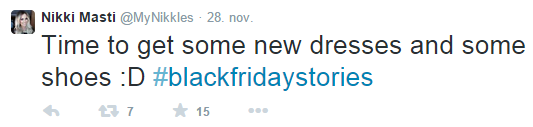
\includegraphics[scale=0.5]{intervention_blackfriday}

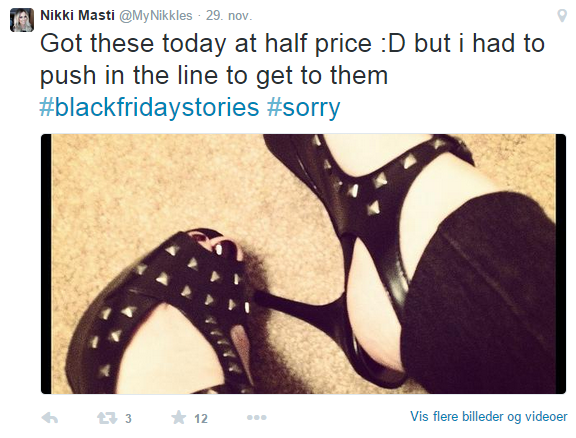
\includegraphics[scale=0.5]{intervention_blackfriday2}

\subsection{Timing Strategy}
Our timing on the tweets, was in such a way, so that we usually made two tweets per day, one in the morning and another tweet once more in the evening. However since the tweets needed to be written manually we saw no reason to create a script which could post it for us. By doing it manually we also gained the advantage of having the tweets look like they were human made.
